% =====================================================================
%  CMAI 2026 — 12-minute oral presentation
%  Solving Bestemshe and Mapping Togyzkumalak
%  Compile:  pdflatex cmai2026.tex   (twice, for the frame counter)
%  Requires: figures/branchingearly.pdf   (slide 4 — the only bitmap/vector import)
% =====================================================================
\documentclass[aspectratio=169]{beamer}
\usetheme{metropolis}
\metroset{background=dark}

\usepackage[utf8]{inputenc}
\usepackage{amsmath,amssymb}
\usepackage{booktabs}
\usepackage{graphicx}
\usepackage{tikz}
\usetikzlibrary{positioning,arrows.meta,calc,shapes.geometric,fit}

% --- Palette -----------------------------------------------------------
% cCyan/cOrange are the categorical pair: validated against the metropolis
% dark surface (#23373B) — lightness band, chroma floor, CVD separation,
% normal-vision floor and contrast all pass.
\definecolor{cCyan}{HTML}{1CA0B4}
\definecolor{cOrange}{HTML}{C2761B}
\definecolor{cGreen}{HTML}{269966}
\definecolor{cRed}{HTML}{D9534F}
\definecolor{cInk}{HTML}{EAEAEA}
\definecolor{cMuted}{HTML}{9BA7A9}

\graphicspath{{figures/}}

% metropolis ships no \framesubtitle template and silently DROPS it;
% render it as a muted lead-in line at the top of the frame body instead.
\renewcommand{\framesubtitle}[1]{%
  {\usebeamerfont{framesubtitle}\color{cMuted}\small #1\par\vspace{3pt}}}

% Monospace code chip for on-screen source lines.
\newcommand{\codechip}[1]{%
  \begin{tikzpicture}[baseline]
    \node[draw=cMuted,rounded corners=2pt,fill=black!25,inner sep=4pt,
          font=\ttfamily\scriptsize,text=cInk] {#1};
  \end{tikzpicture}}

\title{Solving Bestemshe and Mapping Togyzkumalak}
\subtitle{A Mathematical Oracle for Neural Compounding Errors}
\author{Ansar Zeinulla}
\institute{Nazarbayev University}
\date{CMAI 2026}

\begin{document}

% =====================================================================
% PART I — THE HOOK & THE UNCHARTED DOMAIN
% =====================================================================

% --- Slide 1 ---------------------------------------------------------
\begin{frame}[plain]
  \titlepage
\end{frame}

% --- Slide 2 ---------------------------------------------------------
\begin{frame}{The Mancala Frontier}
  \framesubtitle{The missing link in combinatorial complexity}
  \centering
  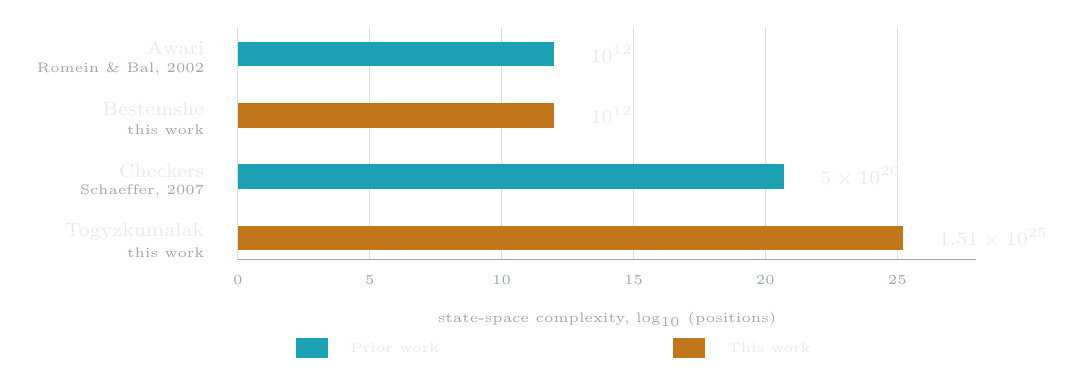
\begin{tikzpicture}[font=\scriptsize, x=0.335cm, y=0.78cm]
    % --- gridlines + axis -------------------------------------------
    \foreach \x in {0,5,10,15,20,25}{
      \draw[cMuted!35,line width=0.3pt] (\x,-0.35) -- (\x,3.42);
      \node[text=cMuted,font=\tiny,anchor=north] at (\x,-0.45) {\x};
    }
    \draw[cMuted] (0,-0.35) -- (28,-0.35);
    \node[text=cMuted,font=\tiny,anchor=north] at (14,-1.05)
      {state-space complexity, $\log_{10}$ (positions)};

    % --- bars: bar length = log10(SSC) -------------------------------
    \foreach \y/\v/\c/\name/\val in {%
        3/12.0/cCyan/{Awari}/{$10^{12}$},
        2/12.0/cOrange/{Bestemshe}/{$10^{12}$},
        1/20.7/cCyan/{Checkers}/{$5\times10^{20}$},
        0/25.2/cOrange/{Togyzkumalak}/{$1.51\times10^{25}$}}
    {
      \fill[\c] (0,\y-0.20) rectangle (\v,\y+0.20);
      \node[anchor=east,text=cInk] at (-0.9,\y+0.10) {\name};
      \node[anchor=west,text=cInk] at (\v+1.0,\y) {\val};
    }
    \node[anchor=east,text=cMuted,font=\tiny] at (-0.9,2.76) {Romein \& Bal, 2002};
    \node[anchor=east,text=cMuted,font=\tiny] at (-0.9,1.76) {this work};
    \node[anchor=east,text=cMuted,font=\tiny] at (-0.9,0.76) {Schaeffer, 2007};
    \node[anchor=east,text=cMuted,font=\tiny] at (-0.9,-0.24) {this work};

    % --- legend, below the axis caption ------------------------------
    \fill[cCyan]   (2.2,-1.95) rectangle (3.4,-1.62);
    \node[anchor=west,text=cInk,font=\tiny] at (3.9,-1.79) {Prior work};
    \fill[cOrange] (16.5,-1.95) rectangle (17.7,-1.62);
    \node[anchor=west,text=cInk,font=\tiny] at (18.2,-1.79) {This work};
  \end{tikzpicture}

  \vspace{0.1cm}
  \begin{itemize}
    \item Bestemshe sits exactly at Awari's complexity --- and is now strongly solved.
    \item Togyzkumalak is five orders of magnitude beyond Checkers.
  \end{itemize}
\end{frame}

% --- Slide 3 ---------------------------------------------------------
\begin{frame}{Mapping Togyzkumalak}
  \framesubtitle{Four structural reductions of the configuration space}
  \centering
  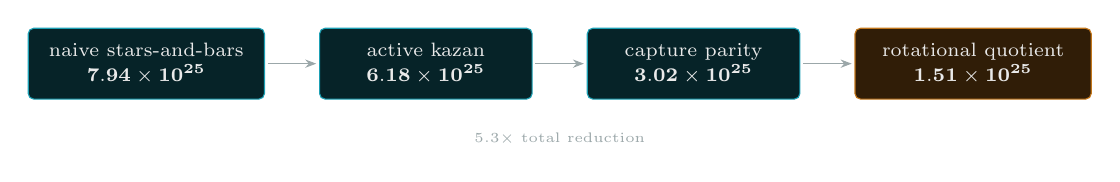
\begin{tikzpicture}[font=\scriptsize,
      stage/.style={draw=cCyan,fill=cCyan!22!black,rounded corners=2pt,
                    text=cInk,minimum height=9mm,align=center,inner xsep=5pt},
      arr/.style={-{Stealth[length=4pt]},cMuted,shorten >=1pt,shorten <=1pt}]
    \node[stage,minimum width=3.0cm] (s0) at (0,0)
      {naive stars-and-bars\\[1pt]$\mathbf{7.94\times10^{25}}$};
    \node[stage,minimum width=2.7cm] (s1) at (3.55,0)
      {active kazan\\[1pt]$\mathbf{6.18\times10^{25}}$};
    \node[stage,minimum width=2.7cm] (s2) at (6.95,0)
      {capture parity\\[1pt]$\mathbf{3.02\times10^{25}}$};
    \node[stage,minimum width=3.0cm,draw=cOrange,fill=cOrange!25!black] (s3) at (10.5,0)
      {rotational quotient\\[1pt]$\mathbf{1.51\times10^{25}}$};
    \draw[arr] (s0) -- (s1);
    \draw[arr] (s1) -- (s2);
    \draw[arr] (s2) -- (s3);
    \node[text=cMuted,font=\tiny] at (5.25,-0.95) {$5.3\times$ total reduction};
  \end{tikzpicture}

  \vspace{0.15cm}
  \begin{equation*}
    \begin{split}
      Z_{\mathrm{unique}} = \frac{1}{2}\Bigg[
        &\sum_{k_1\in E}\sum_{k_2\in E}\binom{R+17}{17}
         + 56\sum_{k_1\in T}\sum_{k_2\in T}\binom{R+15}{15} \\[-2pt]
        &+ 8\Bigg(\sum_{k_1\in T}\sum_{k_2\in E}\binom{R+16}{16}
                 + \sum_{k_1\in E}\sum_{k_2\in T}\binom{R+16}{16}\Bigg)
         + \sum_{k\in E}\binom{89-k}{8}\Bigg]
    \end{split}
  \end{equation*}
  \vspace{-0.2cm}
  {\scriptsize\color{cMuted}
   $R=162-k_1-k_2$;\; $E=\{0,2,\dots,80\}$;\; $T=\{3,\dots,81\}$;\;
   final term $=3.72\times10^{11}$ self-symmetric positions.}
\end{frame}

% --- Slide 4 ---------------------------------------------------------
\begin{frame}{A Billion-Game Empirical Measurement}
  \begin{columns}[T]
    \begin{column}{0.54\textwidth}
      \begin{figure}
        \centering
        \includegraphics[width=\linewidth]{branchingearly.pdf}
      \end{figure}
    \end{column}
    \begin{column}{0.42\textwidth}
      \vspace{0.6cm}
      \begin{itemize}
        \item Empirical GTC \;$\mathbf{10^{105.19}}$
        \item Average game length \;\textbf{124.4 plies}
        \item $10^{9}$ random playouts $\rightarrow$ 124.4B transition counters
      \end{itemize}
      \vspace{0.2cm}
      {\scriptsize\color{cMuted} Branching decays aggressively as material drains, so
       Shannon's static approximation does not hold --- we measured it instead.}
    \end{column}
  \end{columns}
\end{frame}

% --- Slide 5 ---------------------------------------------------------
\begin{frame}{Architecting the Baseline Engine}
  \framesubtitle{Navigating the giant: A 16-byte memory-aligned engine}
  \centering
  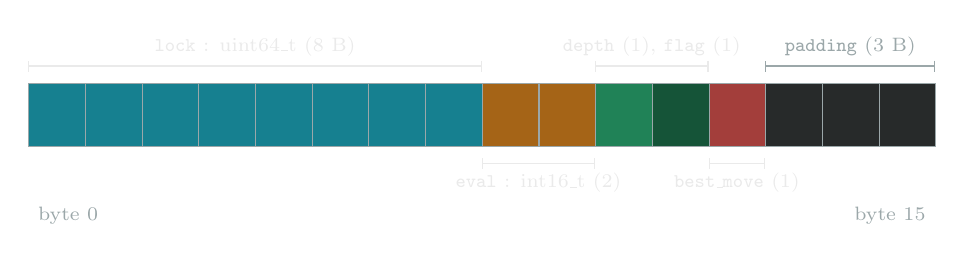
\begin{tikzpicture}[font=\scriptsize,
      byte/.style={draw=cMuted,minimum height=8mm,minimum width=7.2mm,anchor=west}]
    \foreach \i in {0,...,7}
      \node[byte,fill=cCyan!80!black] at (\i*0.72,0) {};
    \node[byte,fill=cOrange!85!black] at (5.76,0) {};
    \node[byte,fill=cOrange!85!black] at (6.48,0) {};
    \node[byte,fill=cGreen!85!black]  at (7.20,0) {};
    \node[byte,fill=cGreen!55!black]  at (7.92,0) {};
    \node[byte,fill=cRed!75!black]    at (8.64,0) {};
    \foreach \i in {13,14,15}
      \node[byte,fill=cMuted!25!black] at (\i*0.72,0) {};

    \draw[cInk,{|[width=4pt]}-{|[width=4pt]}] (0,0.62) -- (5.76,0.62)
      node[midway,above,text=cInk]{\texttt{lock} : uint64\_t (8 B)};
    \draw[cInk,{|[width=4pt]}-{|[width=4pt]}] (5.76,-0.62) -- (7.2,-0.62)
      node[midway,below,text=cInk]{\texttt{eval} : int16\_t (2)};
    \draw[cInk,{|[width=4pt]}-{|[width=4pt]}] (7.2,0.62) -- (8.64,0.62)
      node[midway,above,text=cInk]{\texttt{depth} (1), \texttt{flag} (1)};
    \draw[cInk,{|[width=4pt]}-{|[width=4pt]}] (8.64,-0.62) -- (9.36,-0.62)
      node[midway,below,text=cInk]{\texttt{best\_move} (1)};
    \draw[cMuted,{|[width=4pt]}-{|[width=4pt]}] (9.36,0.62) -- (11.52,0.62)
      node[midway,above,text=cMuted]{\texttt{padding} (3 B)};
    \node[text=cMuted,anchor=west] at (0,-1.28) {byte 0};
    \node[text=cMuted,anchor=east] at (11.52,-1.28) {byte 15};
  \end{tikzpicture}

  \vspace{0.15cm}
  \codechip{static\_assert(sizeof(TTEntry) == 16);}

  \vspace{0.15cm}
  \begin{itemize}
    \item Size is a \emph{compile-time invariant}, guaranteeing no heap fragmentation.
    \item TT-guided ordering: $4.82\text{M}\rightarrow1.43\text{M}$ nodes at depth 9 --- $\mathbf{3.37\times}$ pruning.
    \item \textbf{1.43M NPS} native (Clang++ 17, depth 9, 1.00\,s budget).
  \end{itemize}
\end{frame}

% =====================================================================
% PART II — THE GROUND TRUTH (SOLVING BESTEMSHE)
% =====================================================================

% --- Slide 6 ---------------------------------------------------------
\begin{frame}{Architecting the 8.3\,GB Retrograde Oracle}
  \framesubtitle{The laboratory: Strongly solving the $10^{12}$ variant (Bestemshe)}
  \centering
  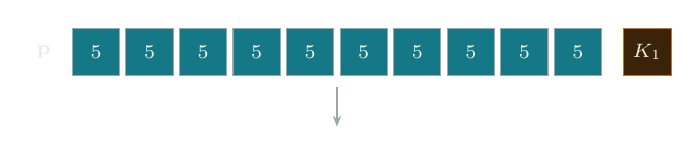
\begin{tikzpicture}[font=\scriptsize,
      pit/.style={draw=cMuted,fill=cCyan!75!black,minimum size=6mm,text=white},
      arr/.style={-{Stealth[length=4pt]},cMuted}]
    \foreach \v [count=\i from 0] in {5,5,5,5,5,5,5,5,5,5}
      \node[pit] (p\i) at (\i*0.68,0) {\v};
    \node[anchor=east,text=cInk] at (-0.45,0) {$\mathbf{p}$};
    \node[draw=cOrange,fill=cOrange!30!black,minimum size=6mm,text=cInk]
      at (7.0,0) {$K_1$};
    \draw[arr] (3.06,-0.45) -- (3.06,-0.95);
  \end{tikzpicture}

  \vspace{-0.1cm}
  \begin{equation*}
    I_B(\mathbf{p}) \;=\; \sum_{i=0}^{8}\binom{\,i+\sum_{j\le i}p_j\,}{\,i+1\,},
    \qquad
    \mathrm{Index}(s) \;=\; I_K\cdot\binom{R+9}{9} \;+\; I_B
  \end{equation*}

  \begin{itemize}
    \item Colexicographical bijection eliminates hash tables entirely. 
    \item $O(1)$ disk-mapped, ZSTD-compressed WDL bitsets --- 169 layers, 338 files.
    \item \textbf{8{,}962{,}782{,}421} bytes; every state lives at a computed mathematical offset.
  \end{itemize}
\end{frame}

% --- Slide 7 ---------------------------------------------------------
\begin{frame}{Game-Theoretic Discoveries: The Greedy Trap}
  \framesubtitle{Verbatim oracle values from the standard start}
  \centering
  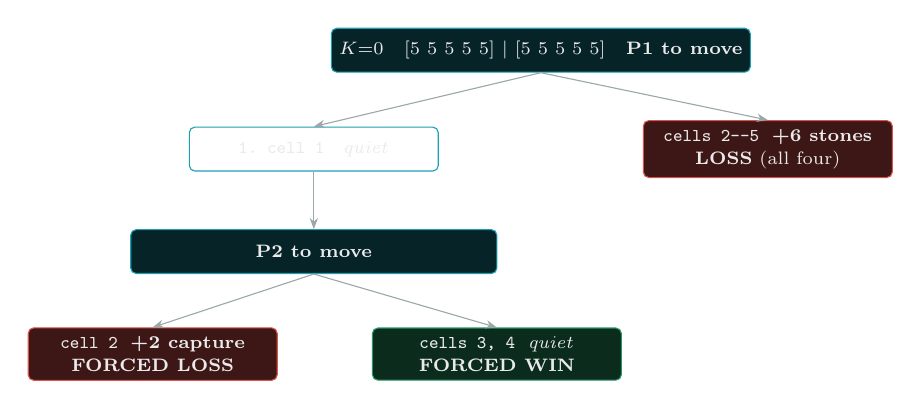
\begin{tikzpicture}[scale=0.93,every node/.style={transform shape},font=\scriptsize,
      nd/.style={draw=cMuted,rounded corners=2pt,minimum height=6mm,minimum width=3.4cm,
                 align=center,text=cInk,inner xsep=3pt},
      state/.style={nd,draw=cCyan,fill=cCyan!22!black,minimum width=5.0cm},
      win/.style={nd,draw=cGreen,fill=cGreen!28!black},
      loss/.style={nd,draw=cRed,fill=cRed!28!black},
      arr/.style={-{Stealth[length=4pt]},cMuted}]

    \node[state] (root) at (0,0)
      {$K{=}0$\quad[5 5 5 5 5] $|$ [5 5 5 5 5]\quad\textbf{P1 to move}};
    \node[nd,draw=cCyan] (q) at (-3.1,-1.35) {\texttt{1.\ cell 1} \;\;\textit{quiet}};
    \node[loss] (grab) at (3.1,-1.35)
      {\texttt{cells 2--5} \;\textbf{+6 stones}\\[1pt]\textbf{LOSS} (all four)};
    \draw[arr] (root.south) -- (q.north);
    \draw[arr] (root.south) -- (grab.north);

    \node[state] (p2) at (-3.1,-2.75) {\textbf{P2 to move}};
    \draw[arr] (q.south) -- (p2.north);

    \node[loss] (c2) at (-5.3,-4.15)
      {\texttt{cell 2} \;\textbf{+2 capture}\\[1pt]\textbf{FORCED LOSS}};
    \node[win]  (c34) at (-0.6,-4.15)
      {\texttt{cells 3, 4} \;\textit{quiet}\\[1pt]\textbf{FORCED WIN}};
    \draw[arr] (p2.south) -- (c2.north);
    \draw[arr] (p2.south) -- (c34.north);
  \end{tikzpicture}

  \vspace{0.15cm}
  {\color{cOrange}\large Structural configuration $>$ material gain.}

  \vspace{0.1cm}
  {\scriptsize\color{cMuted} Four of five first moves capture six stones immediately --- all four are lost.}
\end{frame}

% =====================================================================
% PART III — THE NEURAL BENCHMARK & COMPOUNDING ERROR
% =====================================================================

% --- Slide 8 ---------------------------------------------------------
\begin{frame}{Distilling the Oracle}
  \framesubtitle{Bypassing self-play to learn from mathematical ground truth}
  \centering
  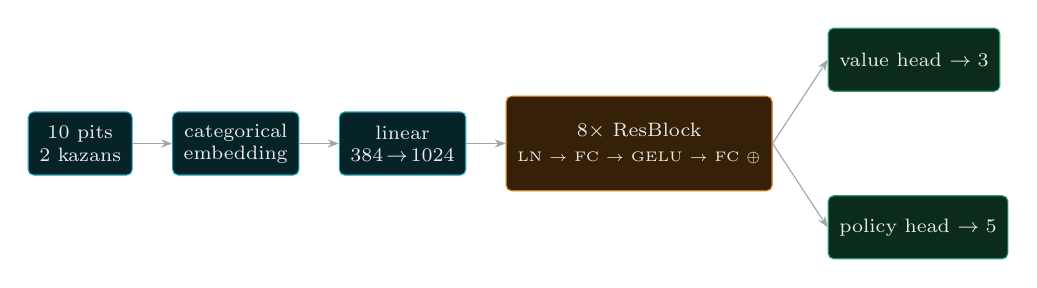
\begin{tikzpicture}[font=\scriptsize,node distance=5mm,
      blk/.style={draw=cCyan,fill=cCyan!22!black,rounded corners=2pt,
                  minimum height=8mm,align=center,text=cInk,inner xsep=4pt},
      arr/.style={-{Stealth[length=4pt]},cMuted}]
    \node[blk] (in) {10 pits\\2 kazans};
    \node[blk,right=of in] (emb) {categorical\\embedding};
    \node[blk,right=of emb] (proj) {linear\\$384\!\to\!1024$};
    \node[blk,draw=cOrange,fill=cOrange!28!black,right=of proj,minimum height=12mm] (body)
      {$8\times$ ResBlock\\[1pt]{\tiny LN $\to$ FC $\to$ GELU $\to$ FC $\oplus$}};
    \node[blk,draw=cGreen,fill=cGreen!28!black,above right=0.5mm and 7mm of body] (v) {value head $\to3$};
    \node[blk,draw=cGreen,fill=cGreen!28!black,below right=0.5mm and 7mm of body] (p) {policy head $\to5$};
    \draw[arr] (in) -- (emb);
    \draw[arr] (emb) -- (proj);
    \draw[arr] (proj) -- (body);
    \draw[arr] (body.east) -- (v.west);
    \draw[arr] (body.east) -- (p.west);
  \end{tikzpicture}

  \vspace{0.35cm}
  \begin{itemize}
    \item \textbf{17.2M parameters} --- AlphaZero-style dual-headed architecture.
    \item \textbf{12.9 billion} configurations presented (394{,}852 steps $\times$ batch 32{,}768).
    \item Targets regenerated directly from the 8.3GB Oracle.
  \end{itemize}
\end{frame}

% --- Slide 9 (NEW) ---------------------------------------------------------
\begin{frame}{The Illusion of AI Evaluation Metrics}
  \framesubtitle{Why 97.48\% optimal-move rate is a forgiving baseline}
  \centering
  \vspace{0.3cm}
  \begin{table}
    \begin{tabular}{lc}
      \toprule
      \textbf{Policy} & \textbf{Optimal-move rate} \\
      \midrule
      Uniform random          & 97.48\% \\
      ResMLP (Our Model)      & \textbf{99.69\%} \\
      \bottomrule
    \end{tabular}
  \end{table}
  \vspace{0.4cm}
  \begin{itemize}
    \item Most positions in Bestemshe are already decisively won or lost.
    \item If a state is a Forced Loss, a random agent cannot make it ``more lost.'' Every move technically preserves the value.
    \item Therefore, 99.69\% actually represents a \textbf{15x reduction} in true boundary-crossing blunders compared to random play.
  \end{itemize}
\end{frame}

% --- Slide 10 ---------------------------------------------------------
\begin{frame}{The Degradation Paradox}
  \framesubtitle{Local accuracy masks global collapse}
  \centering
  \vspace{0.3cm}
  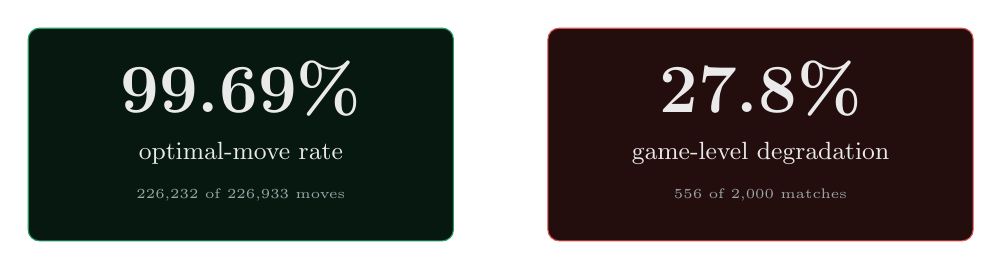
\begin{tikzpicture}[font=\small]
    \node[draw=cGreen,fill=cGreen!16!black,rounded corners=4pt,
          minimum width=5.4cm,minimum height=2.7cm,text=cInk] at (0,0)
      {\begin{tabular}{c}
         {\fontsize{34}{36}\selectfont\textbf{99.69\%}}\\[6pt]
         optimal-move rate\\[3pt]
         {\tiny\color{cMuted} 226{,}232 of 226{,}933 moves}
       \end{tabular}};
    \node[draw=cRed,fill=cRed!16!black,rounded corners=4pt,
          minimum width=5.4cm,minimum height=2.7cm,text=cInk] at (6.6,0)
      {\begin{tabular}{c}
         {\fontsize{34}{36}\selectfont\textbf{27.8\%}}\\[6pt]
         game-level degradation\\[3pt]
         {\tiny\color{cMuted} 556 of 2{,}000 matches}
       \end{tabular}};
  \end{tikzpicture}

  \vspace{0.5cm}
  \begin{itemize}
    \item 2{,}000 matches from forced-symmetric starts against the Oracle.
    \item Near-perfect per move --- yet throws away mathematically won or drawn positions in nearly one game in three.
  \end{itemize}
\end{frame}

% --- Slide 11 --------------------------------------------------------
\begin{frame}{Resolving the Paradox}
  \framesubtitle{The math of compounding failure}
  \begin{equation*}
    P(\text{flawless game}) \;\approx\; p^{L},
    \qquad p = 0.9969, \qquad L = 113
  \end{equation*}
  \begin{equation*}
    (0.9969)^{113} \;\approx\; 0.6960
  \end{equation*}
  \vspace{-0.2cm}
  \begin{center}
    {\color{cOrange}\large \textbf{30.4\%} theoretical failure \quad vs.\quad \textbf{27.8\%} empirical}
  \end{center}
  \vspace{0.1cm}
  \begin{itemize}
    \item The MDP averages 226 plies, requiring exactly 113 independent network decisions.
    \item A 0.31\% per-move error is not small --- it mathematically guarantees global collapse.
    \item The 2.6-point gap is forgiveness: not every blunder crosses a critical value boundary.
  \end{itemize}
\end{frame}

% --- Slide 12 --------------------------------------------------------
\begin{frame}{Conclusion \& Next Steps}
  \vspace{0.4cm}
  \begin{enumerate}
    \setlength{\itemsep}{1.2em}
    \item \textbf{Networks cannot replace search} in deep-tree MDPs. The compounding nature of microscopic errors mathematically guarantees failure.
    \item \textbf{Oracles expose the illusion of Elo ratings} --- per-move accuracy fundamentally hides game-level collapse.
  \end{enumerate}
  \vspace{0.6cm}
  \begin{center}
    {\large Next Step: Multi-threaded tablebase generation for \textbf{weakly solving Togyzkumalak} on unified-memory architectures.}
  \end{center}
  \vspace{0.4cm}
  \begin{center}
    {\color{cOrange}\large Thank you --- questions?}
  \end{center}
\end{frame}

% =====================================================================
% PART IV — HIDDEN DEFENCE MATRIX (BACKUP)
% =====================================================================
\appendix

% --- Slide 13 --------------------------------------------------------
\begin{frame}{Backup: Perft Verification}
  \framesubtitle{Proving the move generator has no silent rule bugs}
  \centering
  \begin{table}
    \begin{tabular}{crl}
      \toprule
      \textbf{Depth $D$} & \textbf{Leaf nodes} & \textbf{Status} \\
      \midrule
      1 & 9        & verified (mathematical limit) \\
      2 & 73       & verified (Allis standard) \\
      3 & 613      & verified (correctness check) \\
      4 & 5{,}199  & verified (system baseline) \\
      \bottomrule
    \end{tabular}
  \end{table}
  \[ \mathrm{Perft}(D,S)=\sum_{m\in\mathcal{M}(S)}\mathrm{Perft}\big(D-1,\mathrm{Step}(S,m)\big),
     \qquad \mathrm{Perft}(0,S)=1 \]
  {\scriptsize\color{cMuted} Counts match the independent exhaustive early-game frontier exactly.}
\end{frame}

% --- Slide 14 --------------------------------------------------------
\begin{frame}{Backup: Memory Safety \& Zobrist Hashing}
  \begin{itemize}
    \item 64-bit Zobrist lock. For $n$ probed states the birthday bound gives
      \[ P(\text{collision}) \;\approx\; 1-e^{-n^{2}/2^{65}} \;\approx\; \frac{n^{2}}{2^{65}} \]
      At $n=2^{24}$ ($16.7$M entries) this is $\approx 7.6\times10^{-6}$.
    \item Always-replace-by-depth write policy:
      \[ \text{Write} \iff (d_{\text{new}} \ge d_{\text{cached}}) \;\lor\; (\text{lock}_{\text{cached}}=0) \]
    \item Wasm scaling: entries $=\big\lfloor \text{MB}\cdot2^{20}/16 \big\rfloor$ floored to a power of
          two, pre-allocated once. $256$\,MB $\rightarrow$ exactly $2^{24}$ slots; the heap
          never grows, so OOM is structurally impossible.
  \end{itemize}
\end{frame}

% --- Slide 15 --------------------------------------------------------
\begin{frame}{Backup: Colexicographical Ranking Derivation}
  For a board $\mathbf{p}=(p_0,\dots,p_9)$ with $M$ stones captured, $R=50-M$ on the board:
  \begin{align*}
    I_B &= \sum_{i=0}^{8}\binom{\,i+\sum_{j\le i}p_j\,}{\,i+1\,}, &
    I_K &= \frac{K_{\text{self}}-\min K(M)}{2}, \\
    \min K(M) &= \max(0,\,M-24), &
    \mathrm{Index} &= I_K\cdot\binom{R+9}{9}+I_B.
  \end{align*}
  \begin{itemize}
    \item Prefix sums make this a bijection onto $\big[0,\binom{R+9}{9}\big)$ --- dense and gap-free.
    \item Capture parity halves the kazan axis: only even increments are reachable.
    \item The inverse is a greedy descent over the same binomials --- no stored table, no hash map.
  \end{itemize}
\end{frame}

% --- Slide 16 --------------------------------------------------------
\begin{frame}{Backup: Proof of the 36-Ply Infinite Cycle}
  \centering
  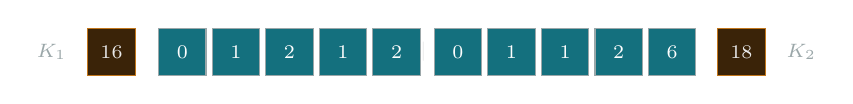
\begin{tikzpicture}[font=\scriptsize,
      pitc/.style={draw=cMuted,fill=cCyan!70!black,minimum size=6mm,text=white},
      kaz/.style={draw=cOrange,fill=cOrange!30!black,minimum size=6mm,text=cInk}]
    \node[kaz] (k1) at (-0.9,0) {16};
    \foreach \v [count=\i from 0] in {0,1,2,1,2}
      \node[pitc] at (\i*0.68,0) {\v};
    \node[text=cInk] at (3.06,0) {$|$};
    \foreach \v [count=\i from 0] in {0,1,1,2,6}
      \node[pitc] at (3.5+\i*0.68,0) {\v};
    \node[kaz] at (7.1,0) {18};
    \node[anchor=east,text=cMuted] at (-1.35,0) {$K_1$};
    \node[anchor=west,text=cMuted] at (7.55,0) {$K_2$};
  \end{tikzpicture}

  \vspace{0.4cm}
  \begin{itemize}
    \item The 36-ply loop is \textbf{capture-free}: $K_1+K_2 = 34$ is constant throughout.
    \item Every capture strictly and irreversibly raises $K_1+K_2$, so no cycle may contain one.
    \item Therefore draws are \emph{not} an artifact of a ply limit --- optimal play genuinely never terminates.
  \end{itemize}
  \vspace{0.2cm}
  {\scriptsize\color{cMuted} Reached after 99 plies of optimal draw-preserving play from the seed position.}
\end{frame}

\end{document}